%%%%%%%%%%%%%%%%%%%%%%%%%%%%% Define Article %%%%%%%%%%%%%%%%%%%%%%%%%%%%%%%%%%
\documentclass{article}
%%%%%%%%%%%%%%%%%%%%%%%%%%%%%%%%%%%%%%%%%%%%%%%%%%%%%%%%%%%%%%%%%%%%%%%%%%%%%%%

%%%%%%%%%%%%%%%%%%%%%%%%%%%%% Using Packages %%%%%%%%%%%%%%%%%%%%%%%%%%%%%%%%%%
\usepackage[utf8]{inputenc}
\usepackage{float}
\usepackage{geometry}
\usepackage{amssymb}
\usepackage{amsthm}
\usepackage{amsmath}
\usepackage{graphicx}
\usepackage[breaklinks]{hyperref}
\usepackage{listings}
\usepackage{fancyhdr}
\usepackage[english]{babel}
\usepackage{mdframed}
\usepackage{lipsum}
\usepackage{color}
\usepackage{psfrag}
\usepackage{pgfplots}
\usepackage{titlesec}
\usepackage{cite}
\usepackage{hyperref}
\usepackage{tabularx}

%%%%%%%%%%%%%%%%%%%%%%%%%%%%%%%%%%%%%%%%%%%%%%%%%%%%%%%%%%%%%%%%%%%%%%%%%%%%%%%

%%%%%%%%%%%%%%%%%%%%%%%%%% C Code Listing Settings %%%%%%%%%%%%%%%%%%%%%%%%%%%%%%%%%%%%%%%
\definecolor{mGreen}{rgb}{0.25,0.63,0.15}
\definecolor{mGray}{rgb}{0.5,0.5,0.5}
\definecolor{mPurple}{rgb}{0.58,0,0.82}
\definecolor{codeBlue}{rgb}{0.01, 0.2, 0.92}
\definecolor{codegray}{rgb}{0.5,0.5,0.5}
\definecolor{codepurple}{rgb}{0.58,0,0.82}
\definecolor{codeblue}{rgb}{0.13,0.29,0.53}
\definecolor{backgroundColour}{rgb}{0.95,0.95,0.95}

\lstset{
    backgroundcolor=\color{backgroundColour},   
    commentstyle=\color{deepGreen},
    keywordstyle=\color{blue},
    numberstyle=\tiny\color{mGray},
    stringstyle=\color{red},
    basicstyle=\ttfamily\small,
    breakatwhitespace=false,
    breaklines=true,
    captionpos=b,
    keepspaces=true,
    numbers=left,
    numbersep=5pt,
    showspaces=false,
    showstringspaces=false,
    showtabs=false,
    tabsize=2,
    language=C,
    frame=single
}


%%%%%%%%%%%%%%%%%%%%%%%%%%%%%%%%%%%%%%%%%%%%%%%%%%%%%%%%%%%%%%%%%%%%%%%%%%%%%%%

% Other Settings
\hypersetup{
    colorlinks = true,
    linkcolor = black,
    urlcolor = blue,
}
\urlstyle{same}

%%%%%%%%%%%%%%%%%%%%%%%%%% Page Setting %%%%%%%%%%%%%%%%%%%%%%%%%%%%%%%%%%%%%%%
\geometry{a4paper}
\pagestyle{fancy}
\fancyhead{}
\fancyhead[L]{CS232 - Operating Systems}
\fancyhead[C]{Assignment 01 - Report}
\fancyhead[R]{}
\fancyfoot{}
\fancyfoot[C]{\thepage}

%%%%%%%%%%%%%%%%%%%%%%%%%% Define some useful colors %%%%%%%%%%%%%%%%%%%%%%%%%%
\definecolor{ocre}{RGB}{243,102,25}
\definecolor{mygray}{RGB}{243,243,244}
\definecolor{deepGreen}{RGB}{26,111,0}
\definecolor{shallowGreen}{RGB}{235,255,255}
\definecolor{deepBlue}{RGB}{61,124,222}
\definecolor{shallowBlue}{RGB}{235,249,255}
%%%%%%%%%%%%%%%%%%%%%%%%%%%%%%%%%%%%%%%%%%%%%%%%%%%%%%%%%%%%%%%%%%%%%%%%%%%%%%%

%%%%%%%%%%%%%%%%%%%%%%%%%% Define an orangebox command %%%%%%%%%%%%%%%%%%%%%%%%
\newcommand\orangebox[1]{\fcolorbox{ocre}{mygray}{\hspace{1em}#1\hspace{1em}}}
%%%%%%%%%%%%%%%%%%%%%%%%%%%%%%%%%%%%%%%%%%%%%%%%%%%%%%%%%%%%%%%%%%%%%%%%%%%%%%%

%%%%%%%%%%%%%%%%%%%%%%%%%%%% English Environments %%%%%%%%%%%%%%%%%%%%%%%%%%%%%
\newtheoremstyle{mytheoremstyle}{3pt}{3pt}{\normalfont}{0cm}{\rmfamily\bfseries}{}{1em}{{\color{black}\thmname{#1}~\thmnumber{#2}}\thmnote{\,--\,#3}}
\newtheoremstyle{myproblemstyle}{3pt}{3pt}{\normalfont}{0cm}{\rmfamily\bfseries}{}{1em}{{\color{black}\thmname{#1}~\thmnumber{#2}}\thmnote{\,--\,#3}}
\theoremstyle{mytheoremstyle}
\newmdtheoremenv[linewidth=1pt,backgroundcolor=shallowGreen,linecolor=deepGreen,leftmargin=0pt,innerleftmargin=20pt,innerrightmargin=20pt,]{theorem}{Theorem}[section]
\theoremstyle{mytheoremstyle}
\newmdtheoremenv[linewidth=1pt,backgroundcolor=shallowBlue,linecolor=deepBlue,leftmargin=0pt,innerleftmargin=20pt,innerrightmargin=20pt,]{definition}{Definition}[section]
\theoremstyle{myproblemstyle}
\newmdtheoremenv[linecolor=black,leftmargin=0pt,innerleftmargin=10pt,innerrightmargin=10pt,]{problem}{Problem}[section]
%%%%%%%%%%%%%%%%%%%%%%%%%%%%%%%%%%%%%%%%%%%%%%%%%%%%%%%%%%%%%%%%%%%%%%%%%%%%%%%

\title{{\huge \textbf{Habib University \\ Operating Systems - CS232 }}

\vspace*{5mm}
{\LARGE \textbf{Assignment 01 - Report}}

% {\Large \textbf{Project Report / Project Title}} \\
{\includegraphics[width=0.75\linewidth]{logo.png}} \\ 
{\Large \textbf{Instructor:} Munzir Zafar}}
\author{Ali Muhammad Asad - aa07190}
\date{}

\pgfplotsset{compat=1.18}

\begin{document}
\maketitle

\newpage
\tableofcontents

\newpage
\section{Introduction}
The assignment is to simulate a simple file system in C language. The file system is simulated using a single file \textbf{``myfs''} which acts as the hard disk. The whole disk is 128KB in size, has the root directory \textbf{``/''}, and can have a maximum of 16 files/directories (therefore 16 inodes). A file can have a maximum of 8 blocks, each of size 1KB. 

\section{Disk Layout}
The disk is divided into 128 blocks, each of size 1KB. The first block is the super block, and the rest 127 blocks are the data blocks. The super block contains the 128 byte free block list where each byte contains a boolean value indicating whther that particular block is free or not. Just after the free block list, the inodes are stored - in total there are 16 inodes, where each inode corresponds to one file or directory. Each inode is 56 bytes into size and contains the metadata about the stored files/directories. The contents of the directory are a series of directory entries comprising of dirent structures (will be further explained later on). The disk layout can be visually represented as follows:
\begin{figure}[htbp]
    \centering
    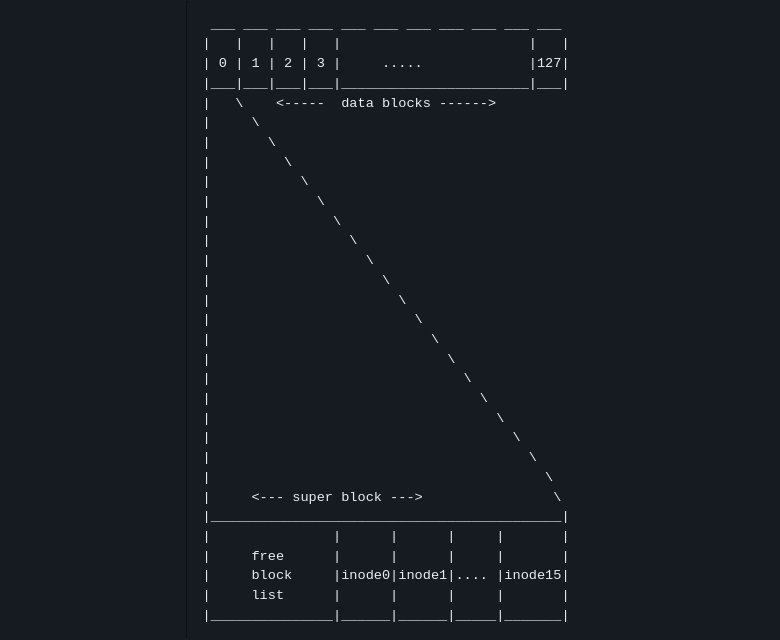
\includegraphics[width=0.9\textwidth]{disk_layout.png}
    \caption{Disk Layout}
    \label{fig:disk_layout}
\end{figure}

\newpage
\section{Input and Makefile}
\subsection{Input}
The program takes a command line argument which will be a file containing the commands to be executed. The commands are read by the program and executed one by one, and each command should be on a separate line. The input should always be in the correct format, i.e., \texttt{Command Arg1 Arg2} or \texttt{Command Arg}, otherwise the program will not work as expected. The input file should be in the same directory as the program. 

\subsection{Makefile}
The accompanying makefile has also been provided with the program. The makefile supports the following commands: \vspace*{-2mm}
\begin{itemize}
    \item[-] \texttt{make build:} builds the program and creates the executable file titled \textbf{``myfs.out''}.
    \item[-] \texttt{make run:} runs the program with the default input file \textbf{``sampleinput.txt''}. The input file can be changed to any other file as needed. Running the program will also create the \textbf{``myfs''} file which acts as the hard disk.
    \item[-] \texttt{make clean:} cleans the directory by removing the executable file (``myfs.out'') and the disk file (``myfs'').  
\end{itemize}

\newpage
\section{Implementation}
\subsection{Data Structures}
There are several data structures that are being used in this implementation to manage and store the ``myfs'' filesystem's data and key components.

\begin{enumerate}
    \item \textbf{Super Block:} The super block, although not explicitly defined as a data structure, can be conceptually understood as a data structure storing the first few bytes of the \textbf{``myfs''} filesystem. The super block is stored in the first block of the disk and contains critical information about the file system such as the identification marker ``A'' (corresponding to the initial of my name as I implemented this file system) and the directory bitmap ``1''.
    
    It contains the free block list and the inodes. The free block list is an array of 128 bytes, where each byte represents a block in the disk. If the value of the byte is 0, then the block is free, otherwise it is not. The inodes are an array of 16 inodes, where each inode corresponds to a file or directory.

    \item \textbf{Inode (struct inode):} The inode is a data structure - implemented using a struct - that stores the metadata of a file or directory. In my implementation, there are 16 inodes, stored consecutively in the disk just after the free block list in the file system. Inividual inodes are accessed using the \texttt{lseek} function to the appropriate position, followed by a subsequent read or write operation. Each inode is 56 bytes in size, and is defined as follows containing the following information:
    \begin{lstlisting}[caption={Inode Structure}, label={lst:inode}]
typedef struct inode {
    int dir;                    // 1: directory, 0: file
    char name[FILENAME_MAXLEN]; // File / directory name
    int size;                   // File / directory size in bytes
    int blockptrs[8];           // Direct pointers to data blocks
    int used;                   // 1 if the entry is in use
    int rsvd;                   // Reserved for future use
} inode;
    \end{lstlisting}

    \item \textbf{Directory Entry (struct dirent:)} The directory entry or \textit{dirent} for short, is a data structure - implemented using a struct - that stores the information about a file or directory within a directory. These entries are stored within data blocks. Similar to the inodes, individual directory entries are accessed using the \texttt{lseek} function to the appropriate position, followed by a subsequent read or write operation. Each directory entry is 32 bytes in size, and is defined as follows containing the following information:
    \begin{lstlisting}[caption={Dirent Structure}, label={lst:directory_entry}]
typedef struct dirent {
    char name[FILENAME_MAXLEN]; // Name of the entry
    int namelen;                // Length of entry name
    int inode;                  // Index of the corresponding inode
} dirent;   
    \end{lstlisting}

    \item \textbf{Data Blocks:} Data blocks store the actual content of files and directories. Again, the data blocks are accessed using the \texttt{lseek} function to the appropriate position, followed by a subsequent read or write operation. Each data block is 1KB in size, made as 127 blocks in the disk. The data blocks are accessed using the blockpointers in the inode. The blockpointers are an array of 8 integers. The data blocks can be conceptually visualized as shown in Figure \ref{fig:disk_layout}.
    
    \item \textbf{MYFS - My File System:} The ``myfs'', although a file, is the fundamental data structure in the implementation, serving as the underlying storage medium that imitates the hard disk. ``myfs'' is where all the file system data is stored. A function ``\texttt{init()}'' initializes the file system which is shown below in Listing \ref{lst:init}. Then the function is called in the main function, which returns the file descriptor of the file system. The file descriptor is then used to access the file system. The file system is then accessed using the \texttt{lseek} function to the appropriate position, followed by a subsequent read or write operations.
\end{enumerate}

\newpage
\subsection{Algorithms and Code}

There is no specific algorithm that was followed to implement the file system. The implementation was done in a very simple fashion, where the file system was first initialized, then the subsequent functions, and data structures were created, followed by the main function where the initialization was done, and the input file was parsed line by line. In general, the algorithm followed the following pattern: \\ 
\hspace*{5mm} - use \texttt{lseek} to seek over to the required inode, or the directory entry, or the data block \\
\hspace*{5mm} - use \texttt{read} or \texttt{write} to read or write the required data

\noindent A function ``\texttt{init()}'' initializes the file system:
    \begin{lstlisting}[caption={Initialization of MYFS}, label={lst:init}]
int init(){
    int myfs = open("./myfs", O_CREAT | O_RDWR, 0666); // create a file named myfs with read write enabled
    if(myfs == -1){
        printf("Error: Cannot create file system myfs\n"); return -1;
    }

    ftruncate(myfs, BLOCK_SIZE * NUM_BLOCKS); // 128 * 1024 = 128KB allocated to myfs

    // identification and directory bitmap
    char fs = 'A'; write(myfs, (char*)&fs, 1);
    char dbm = (char)1; write(myfs, (char*)&dbm, 1);

    // Initializing the Root Inode
    struct inode root_inode;
    root_inode.dir = 1; // root inode is a directory
    strcpy(root_inode.name, "/"); // first root directory named "/"
    root_inode.size = sizeof(struct dirent);
    root_inode.blockptrs[0] = 1;
    root_inode.used = 1; // yes it is in use
    root_inode.rsvd = 0; // no it is not reserved for future use
    
    // write the root inode into myfs
    lseek(myfs, NUM_BLOCKS, SEEK_SET); 
    write(myfs, (char*)&root_inode, sizeof(struct inode));

    // Initializing the Root Directory Entry
    struct dirent root_dirent;
    strcpy(root_dirent.name, ".");
    root_dirent.namelen = 1;
    root_dirent.inode = 0;

    // write the root directory entry into myfs
    lseek(myfs, BLOCK_SIZE, SEEK_SET); 
    write(myfs, (char*)&root_dirent, sizeof(struct dirent));

    return myfs;
}
\end{lstlisting}
In the above listing, ``myfs'' is first opened as a file, with read and write permissions enabled. If there's any issue in creating the file system, an error message is thrown and the function exits. If the file is created successfully, the file is truncated to 128KB in size. The first two bytes of the file are then written with the identification marker ``A'' and the directory bitmap ``1''. The root inode is then initialized and written into the file system. The root inode is a directory, and has the name ``/''. The size of the root inode is the size of a single directory entry. The root inode has a single block pointer, which points to the first data block. The root inode is then written into the file system. \\ The root directory entry is then initialized and written into the file system. The root directory entry has the name ``.'', and the inode number of the root inode. The root directory entry is then written into the file system. The function then returns the file descriptor of the file system, which is then used to access the file system.


The \texttt{main} function is responsible for opening the ``myfs'' file system, and parsing over the input file. This \texttt{main} serves as the control center of the file system implementation, by first creating the file system if it does not exist, and then parsing over the input file line by line. The command is parsed using the \texttt{sscanf} function, and then the appropriate function is called. The input file is parsed line by line using the \texttt{getline} function. The \texttt{getline} function returns -1 when the end of the file is reached. The \texttt{getline} function also allocates memory to the line variable, which is freed at the end of the program. The input file is opened using the \texttt{fopen} function, and is closed at the end of the program. The file system is opened using the \texttt{open} function, and is closed at the end of the program.
% The main function is shown below:
% \begin{lstlisting}[caption={Main Function}, label={lst:main}]
% int main(int argc, char* argv[]){
%     myfs = open("./myfs", O_RDWR); // open file "myfs" with rw access
%     if(myfs == -1) myfs = init(); // if file does not exist, create it

%     FILE *stream = fopen(argv[1], "r"); // open input file
%     if(stream == NULL){ // if file does not exist, throw an error
%         printf("Error opening file\n"); exit(1);
%     }

%     // variables to hold the input line and the command
%     char* line = NULL; char command[3]; size_t len = 0;

%     // parse over the input file line by line
%     while(getline(&line, &len, stream) != - 1){
%         sscanf(line, "%s %[^\n]", command, line); // parse the command and the rest of the line
%         if(strcmp(command, "CR") == 0){ // create a file
%             char* filename = strtok(line, " ");
%             int size = atoi(strtok(NULL, " "));
%             CR(filename, size);
%         }
%         else if(strcmp(command, "DL") == 0){ // delete a file
%             DL(line);
%         }
%         else if(strcmp(command, "CP") == 0){ // copy a file
%             char* srcname = strtok(line, " "), *dstname = strtok(NULL, " ");
%             CP(srcname, dstname);
%         }
%         else if(strcmp(command, "MV") == 0){ // move a file
%             char* srcname = strtok(line, " "), *dstname = strtok(NULL, " ");
%             MV(srcname, dstname);
%         }
%         else if(strcmp(command, "CD") == 0){ // create a directory
%             line = strtok(line, "\n"); CD(line);
%         }
%         else if(strcmp(command, "DD") == 0){ // delete a directory
%             DD(line);
%         }
%         else if(strcmp(command, "LL") == 0){ // list all files
%             LL();
%         }
%     }
%     // free memory allocated to line, close the input file and the file system
%     free(line); fclose(stream); close(myfs); 
%     return 0;
% }
% \end{lstlisting}



\newpage
\section{Takeaway and Reflection}
While doing this assignment, the sheer dedication, will power, sleepless nights and the amount of time and effort that goes into making a file system was realized. The assignment was a great learning experience, and I learned a lot about how file systems work (in a very simple fashion though, not too complex). I also learned that I have much more patience than I realized to not completely give up while understanding the implementation, not to mention the fact that twice I had to completely start from scratch due to lack of understanding and wrong implementation, and once more because my whole system crashed due to an error I still don't know about. This assignment seemed nothing less than a project to me, and I am glad I was able to complete it (in whatever state it is currently in). I would not want to indulge in this ever again. The image attached below sums up my emotions, reflections and feelings during and after the assignment.

\begin{figure}[htbp]
    \centering
    
\includegraphics[width=\textwidth]{takeaway.jpg}
\end{figure}

\newpage
\section{References}
\begin{thebibliography}{9}
    \bibitem{github}
    \textit{GitHub}. \hspace*{-1mm}[Online]. \hspace*{-1mm}Available: \hspace*{-2mm}\url{https://github.com/bartooo/very-simple-file-system/blob/main/main.c}

    \bibitem{Github}
    \textit{GitHub}. \hspace*{-1mm}[Online]. \hspace*{-1mm}Available: \hspace*{-2mm}\url{https://github.com/Luminoid/Simple-File-System}

    \bibitem{GitHub}
    \textit{GitHub}. \hspace*{-1mm}[Online]. \hspace*{-1mm}Available: \hspace*{-2mm}\url{https://github.com/jcbbeiter/simple-file-system}
    
    \bibitem{gitHub}
    \textit{GitHub}. \hspace*{-1mm}[Online]. \hspace*{-1mm}Available: \hspace*{-2mm}\url{https://github.com/paleumm/vsfs/blob/main/src/block.c}

    \bibitem{}
    \textit{GitHub}. \hspace*{-1mm}[Online]. \hspace*{-1mm}Available: \hspace*{-2mm}\url{https://github.com/SrLozano/Simple-File-System/blob/master/filesystem/filesystem.c}


    \bibitem{chatgpt}
    OpenAI. \textit{ChatGPT} [Online]. Available: \hspace*{-2mm} \url{https://chat.openai.com/} mainly for understanding, error resolving, and commentation.
\end{thebibliography}

\appendix
\section{Appendix}
The file system has been uploaded on to my repository on GitHub. The repository can be accessed through the following link: \url{https://github.com/AliMuhammadAsad/A-Simple-File-System/}

\end{document}